\section{Background}\label{sec:background}
Neural machine translation~(NMT) is formulated as a conditional probability model $p(\y|\x)$, which models a sentence $\y = \{y_1,y_2,\cdots,y_m\}$ in the target language given the input $\x = \{x_1,x_2,\cdots,x_n\}$ from the source language.
% where $n$ and $m$ are the length of the source and target sentence, respectively. 

% \subsection{Autoregressive Neural Machine Translation}\label{ss:auto}
% Deep neural networks with autoregressive encoder-decoder framework achieves great success on machine translation~\cite{rnn_search}. 
% For a target sentence $y=\{y_1,y_2,\cdots,y_m\}$, an autoregressive decoder factorizes its probability into a series of conditional probabilities, given the source sentence $x=\{x_1,x_2,\cdots,x_n\}$:
% \begin{equation}
%     p(y|x) = \prod_{t=1}^{m} p(y_{t}|y_{<t},x;\theta),
%     \label{eqn:at}
% \end{equation}
% where $\theta$ is a set of model parameters and $y_{<t}$ is the translation history. 

% Autoregressive models such as CNN~\cite{cnn_seq} and Transformer~\cite{transformer} could be parallelized during training thanks to the nature of teacher-forcing.
% However, they suffer from slow decoding due to the autoregressive restriction to predict the token by given previously generated outputs~(see Figure~\ref{fig:at}).

\subsection{Non-Autoregressive Neural Machine Translation}\label{ss:non-auto}
\citet{nat} proposes Non-Autoregressive Transformer~(NAT) for machine translation, breaking the dependency among target tokens, thus achieving simultaneous decoding for all tokens. 
For a source sentence, a non-autoregressive decoder factorizes the probability of its target sentence as:
\begin{equation}
    p(\y|\x)= \prod_{t=1}^{m}p(y_{t}|\x; \theta),
    \label{eqn:nat}
\end{equation}
where $\theta$ is the set of model parameters.

NAT has a similar architecture to the autoregressive Transformer~\citep[AT,][]{transformer}, which consists of a multi-head attention based encoder and decoder. 
The model first encodes the source sentence $x_{1:n}$ as the contextual representation $e_{1:n}$, then employs an extra module to predict the target length and form the decoder inputs.
% However, the NAT model has no explicitly previous outputs as the decoder input, neither has the sequently generated token \texttt{<EOS>} to implicitly decide the target length. 
% The common practice in NAT models is to set an extra bridge module to predict the target length and form the decoder inputs. 
\begin{itemize}
    \item \textbf{Length Prediction: } Specifically, the length predictor in the bridge module predicts the target sequence length $m$ by:
    \begin{equation}
        m = n + \argmax_{\Delta L} p(\Delta_{L}|\operatorname{mean}(e); \phi),
    \end{equation}
    where $\Delta_{L}$ is the length difference between the target and source sentence, $\phi$ is the parameter of length predictor.
    \item \textbf{Inputs Initialization: } With the target sequence length $m$, we can compute the decoder inputs $\h=h_{1:m}$ with \textit{Softcopy}~\cite{hint_nat,imitate_nat} as:
    \begin{equation}
        \begin{split}
          h_j & = \sum_{i}^{n} w_{ij}\cdot e_i  \\
        \text{and}\ w_{ij} & = \softmax (-|j-i|/\tau),
    \end{split}
    \label{equ:softcopy}
    \end{equation}
    where $\tau$ is a hyper-parameter to control the sharpness of the $\softmax$ function.
\end{itemize}
% \pseudopara{Length Prediction } 
% \paragraph{Length Prediction.} 
% Specifically, the length predictor in the bridge module predicts the target sequence length $m$ by:
% \begin{equation}
%   m = n + \argmax_{\Delta L} p(\Delta_{L}|\operatorname{mean}(e); \phi),
% \end{equation}
% % $m = n + \argmax p(\Delta_{L}|\operatorname{mean}(e); \phi)$, 
% where $\Delta_{L}$ is the length difference between the target and source sentence, $\phi$ is the parameter of length predictor.
% \paragraph{Decoder Inputs.}
% With the target sequence length $m$, we can compute the decoder inputs $h$ with \textit{Softcopy}~\cite{hint_nat,imitate_nat} as:
% \begin{equation}
%     \begin{split}
%           h_j & = \sum_{i}^{n} w_{ij}\cdot e_i  \\
%     \text{and}\ w_{ij} & = \softmax (-|j-i|/\tau), \\
%     \end{split}
% \label{equ:softcopy}
% \end{equation}
% where $\tau$ is a hyper-parameter to control the sharpness of the $\softmax$ function. 
With the computed decoder inputs $h$, NAT generates target sequences simultaneously by $\argmax_{y_t}\ p(y_t|x; \theta)$ for each timestep $t$, effectively reduce computational overhead in decoding~(see Figure~\ref{fig:nat}). 

Though NAT achieves around $10\times$ speedup in machine translation than autoregressive models, it still suffers from potential performance degradation~\citep{nat}.
The results degrade since the removal of target dependencies prevents the decoder from leveraging the inherent sentence structure in prediction.
Moreover, taking the copied source representation as decoder inputs implicitly assume that the source and target language share a similar order, which may not always be the case~\cite{pnat}.
% Besides, the copied source representation may not be the best to the non-autoregressive decoding~\cite{enat,pnat}, since it assume that the source language and target language always has the similar order.
% Without such dependencies, the decoder is hard to leverage the inherent sentence structure in prediction.
% The potential modeling gap between the underlying, true model and the neural sequence model, could be larger with the non-autoregressive model compared to the autoregressive one due to challenge of modeling the factorized conditional distribution above\citep{iter_nat}.

\begin{figure}[tbp]
    \centering
    \small
    \begin{minipage}{0.3\linewidth}
    \centering
    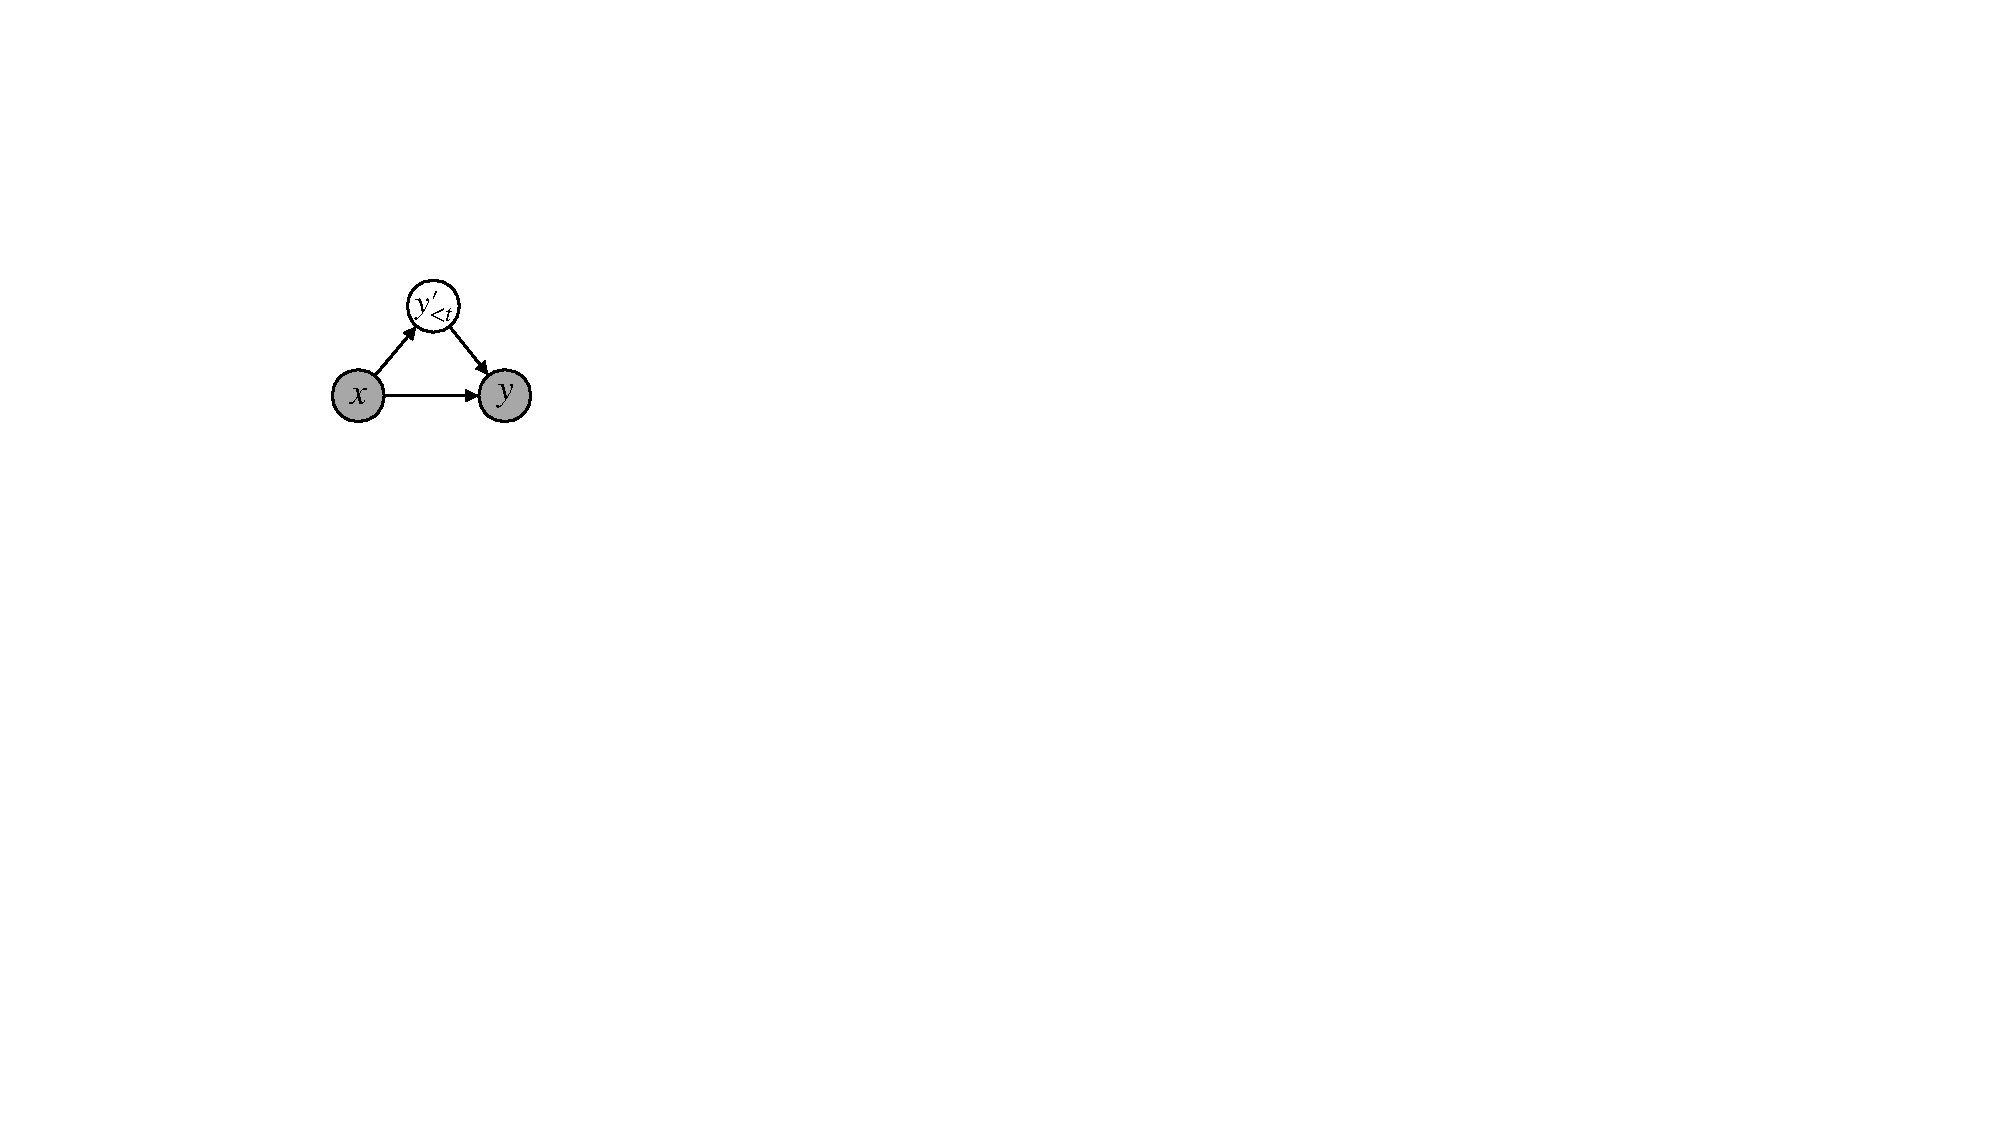
\includegraphics[width=\linewidth]{figures/AT-Inference.pdf}
    \subcaption{AT}
    \label{fig:at}
    \end{minipage}
    \hfill
    \begin{minipage}{0.3\linewidth}
    \centering
    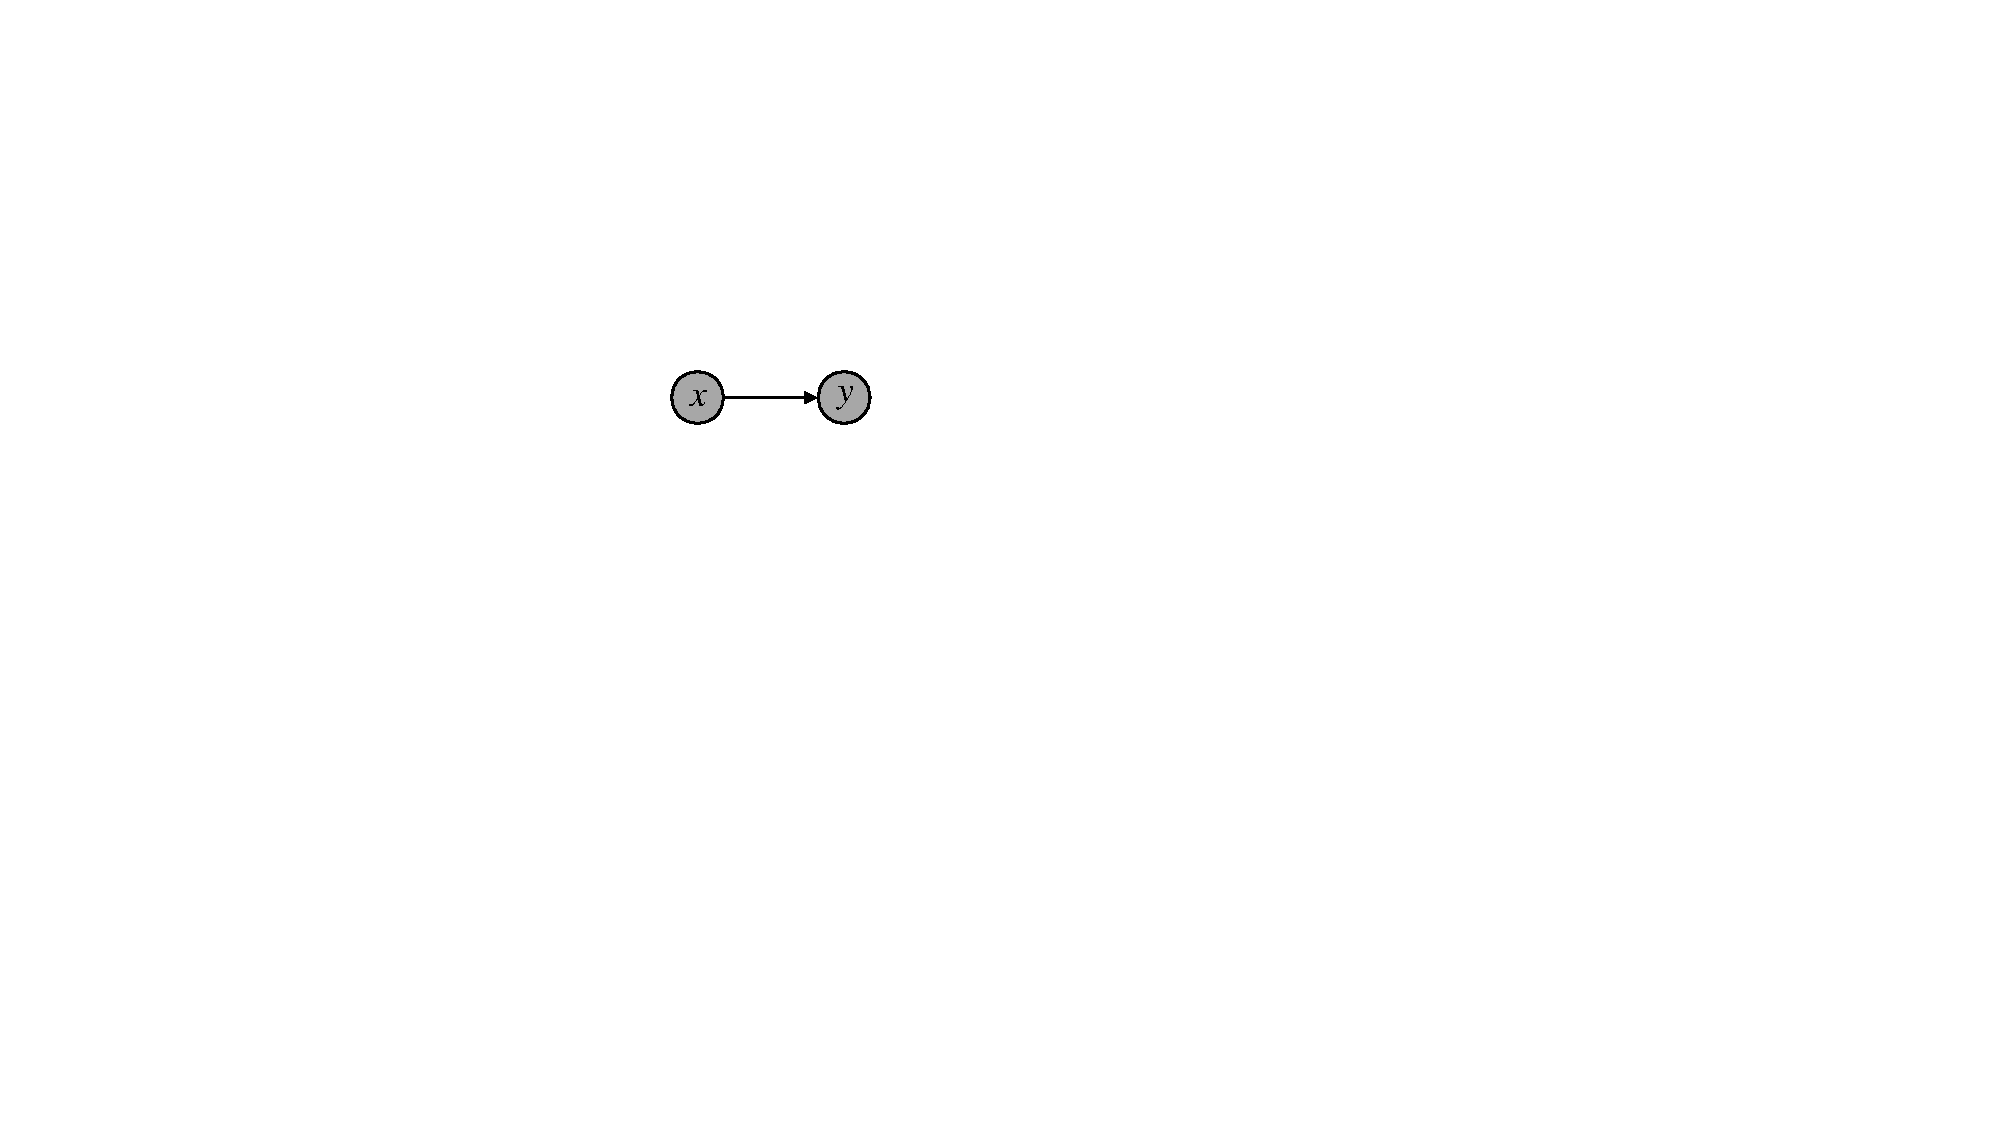
\includegraphics[width=\linewidth]{figures/NAT-Decoding.pdf}
    \subcaption{NAT}
    \label{fig:nat}
    \end{minipage}
    \hfill
    \begin{minipage}{0.3\linewidth}
    \centering
    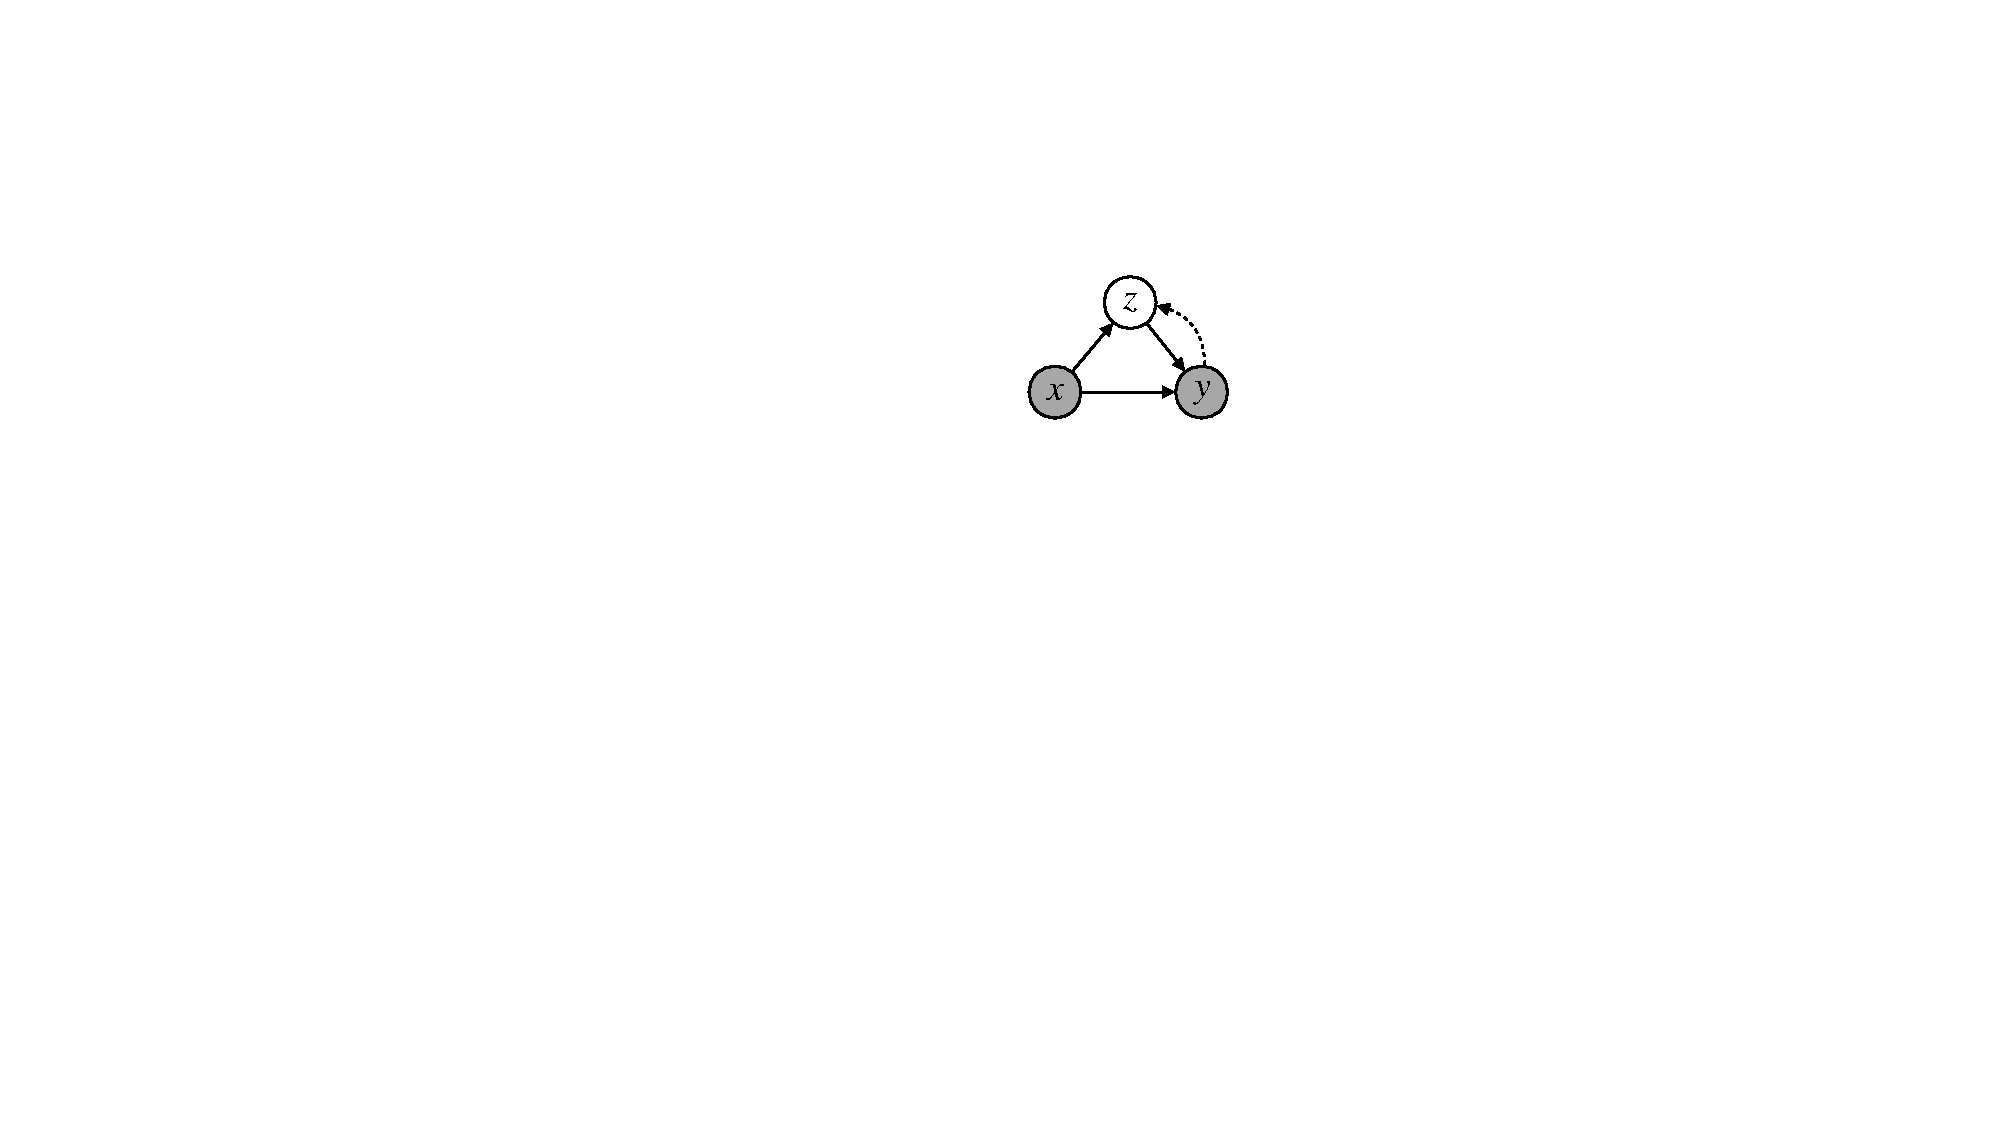
\includegraphics[width=\linewidth]{figures/LT-Decoding.pdf}
    \subcaption{LT}
    \label{fig:lt}
    \end{minipage}
\caption{Different inference process of different Transformer models.}
\label{fig:lm}
\end{figure}

\subsection{Latent Transformer}\label{ss:latent-nat}
To bridge the gap between non-autoregressive and autoregressive decoding, \citet{lt} introduce the Latent Transformer~(LT).
It incorporates non-autoregressive decoding with conditional dependency as the latent variable to alleviate the degradation resulted from the absence of dependency:
% \begin{equation}
% \label{eqn:lt}
    % p(y|x)= \int_{\z} p(\z|x;\phi) \prod_{t=1}^{m} p(y_{t}|\z,x; \theta)dz,
% \end{equation}
\begin{equation}
\label{eqn:lt}
    p(\y|\x)= p(\z|\x;\phi) \prod_{t=1}^{m} p(y_{t}|\z,\x; \theta),
\end{equation}
where $\z=\{z_1,\cdots,z_L\}$ is the latent sequence and the $L$ is the length of the latent sequence, $\phi$ and $\theta$ are the parameter of latent predictor and translation model, respectively. 

The LT architecture stays unchanged from the origin NAT models, except for the latent predictor and decoder inputs. 
During inference, the Latent Transformer first autoregressively predicts the latent variables $\z$, then non-autoregressively produces the entire target sentence $\y$ conditioned on the latent sequence $\z$~(see Figure~\ref{fig:lt}). \citet{flowseq,lv_nar} extend this idea and model $\z$ as the continuous latent variables, achieving a promising result, which replaces the autoregressive predictor with the iterative transformation layer.
% ~\citet{syn_st} introduces the syntactic information as a proxy to the learned discrete latent space of the LT and improves the performance. 
% Although the Latent Transformer outperforms the vanilla NAT, it remains the following issues:
% \begin{itemize}
%     \item relying on a large value of latent codes~($> 2^{16}$ latents in~\citealp{lt}) or multiple iterative layer~(around 30 inevitable transformation layer in~\citealp{flowseq}), which may hurt translation efficiency,
%     \item autoregressive decoding for latent sequences potentially leads to a mismatch of the training and inference in~\citet{lt}, which may hurt translation quality.
% \end{itemize}

% Although the Latent Transformer outperforms the vanilla NAT, it still relying on a large value of latent codes~($> 2^{16}$ latents in~\citealp{lt}) or multiple iterative layer~(around 30 inevitable transformation layer in~\citealp{flowseq}), which may hurt translation efficiency,